
\begin{dialog}{和声小迷宫}

\begin{quote}
乌龟和阿基里斯在游乐场玩了一天。他们先买了一对棉花糖,然后决定去乘“大风车”玩。
\end{quote}

\setnamewidth{2\ccwd}

\begin{dialogue}

\item[乌龟]这是我最喜欢的游艺项目。坐在上面你感觉似乎移动了很远,其实仍在原地。

\item[阿基里斯]我知道它为什么叫你着迷。你系好安全带了吗?

\item[乌龟]好啦,我觉得我把这扣子扣好了。哎,开始吧。喔!

\item[阿基里斯]你今天很兴奋吧。

\item[乌龟]这是有缘故的。我姑妈会算命,她对我说今天我会遇到好运。正是因为期待着那个好运我才这么兴奋的。

\item[阿基里斯]你居然相信算命!

\item[乌龟]不……但是人们说即使你不信,它也一样灵。

\item[阿基里斯]哼,要真是这样倒不错。

\item[乌龟]啊,风景多美啊。你看这片海滩、海边上游泳的人们、蓝色的大海、还有这座城市……

\item[阿基里斯]对,的确美不胜收。喂,瞧那边那架直升飞机,似乎朝我们这儿飞来了。现在它实际上几乎就在我们头顶上了。

\item[乌龟]怪事——飞机上还垂下一条缆绳来,离我们非常近。我们只要伸手就能抓得到。

\item[阿基里斯]瞧!那条缆绳的头儿上有个大钩子,上面挂着一张纸条。

\dnote{(他伸手抓下纸条。旋转着的大风车带着他们转了下去。)}

\item[乌龟]你能认出条上写的什么吗?

\item[阿基里斯]能——写的是,“你们好,朋友们。再转上来的时候抓住钩子,会叫你们喜出望外的。”

\item[乌龟]条子上写的跟游艺场广告上的陈词滥调一个味儿,不过谁知道这意味着什么。也许跟我要遇到的好运有关。不管怎么着,我们得试试!

\item[阿基里斯]得试试!

\dnote{(“大风车”把他们转上来的时候,他们两个都解开了安全带的系扣。当转到最高点时,他们抓住了那个巨大的钩子,缆绳马上把他们悠起来,一直绞向悬在空中的直升飞机。一只粗大有力的手帮他们进了飞机。)}

\item[声音]欢迎登机——两位冒失鬼。

\item[阿基里斯]你——你是谁?

\item[声音]请允许我自我介绍一下:我是郝晕,逍遥自在的拐子,最优秀的噬龟者,听候二位的吩咐。

\item[乌龟]哎呀!

\item[阿基里斯\dlnote{(对他的朋友低语)}]唔——哦——我看这位“郝晕”真不是我们期待的那个。\dlnote{(对郝暈说)}哎——如果我可以如此大胆的话——你这是要把我们拐到哪儿去啊?

\item[郝晕]哈哈!去我的全电气化空中厨房,在那儿我要把这位做成有滋有味的小点心——\dlnote{(他说这话的时候,瞟了乌龟一眼)}——做成美味可口的天上馅饼!没错儿——拿来满足我的饕餮之欲!哈哈哈!

\item[阿基里斯]我只能说你的笑声像恶魔一样。

\item[郝晕]\dlnote{(恶魔般地大笑)}哈哈哈!你竟敢这么放肆!朋友,有你好瞧的。哈哈!

\item[阿基里斯]天哪!他这话是什么意思!

\item[郝晕]很简单——我给你们二位准备了恶运!你们等着吧!哈哈哈!哈哈哈!

\item[阿基里斯]糟啦!

\item[郝晕]好,我们到了。下机吧,朋友们,到我那绝妙的全电气化空中厨房里来吧。

\dnote{(他们走进去。)}

在你们倒霉之前,让我带着你们先参观参观。这是我的卧室,这是我的书房。请先在这儿等我一会儿,我得去磨磨我的刀子。你们可以边等边吃点“弹出锅酥”。哈哈哈!乌龟馅!乌龟馅!我最喜欢的一种馅!\dlnote{(走开了。)}

\item[阿基里斯]喔,天哪——弹出锅酥!我可得甩开腮帮子足吃!

\item[乌龟]阿基!你可是刚刚大嚼了一通棉花糖啊!况且,这种时候你怎么还想吃东西?

\item[阿基里斯]糟糕——哦,真对不起——我不应该用带有“糕”这种食品名称的词,我是想说在这样不幸的时候……

\item[乌龟]我想恐怕我们都得引颈就戮了。

\item[阿基里斯]是啊——你是应该翘首引颈好好瞧瞧郝晕那家伙书房里的那些书。那是些什么书啊——哦,原来是孤本书大全:《我所认识的呆瓜》、《象棋和转伞安然相处》、《为踢踏舞和管弦乐队写的协奏曲》……哼!

\item[乌龟]书桌上放着一本什么书啊?紧挨着那个十二面体和打开的速写本?

\item[阿基里斯]这本吗?喔,书名是《阿基里斯和乌龟在全球瞎逛时引人入胜的历险》。

\item[乌龟]名字有点吸引人呢。

\item[阿基里斯]的确——而且这页上的故事看上去也很吸引人。故事的名字是《神怪和煮调饮》。

\item[乌龟]冷饮?

\item[阿基里斯]不是,是“煮调饮”,大概是一种煮着喝加调料的饮料吧?我也不懂。

\item[乌龟]哼……怪事。我们读读它好吗?我读乌龟的台词,你当阿基里斯。

\item[阿基里斯]行啊。干嘛不呢……

\dnote{(他们开始阅读《神怪和煮调饮》。)}

  \begin{dialogue}

  \item[]\dnote{(阿基里斯邀请乌龟来欣赏他收集的他最喜欢的画家艾舍尔的作品。)}

  \item[乌龟]这些画好极了,阿基。

  \item[阿基里斯]我知道你会喜欢的。你最喜欢哪一幅?

  \item[乌龟]我最喜欢的一幅是《凹与凸》,在那幅画中有两个在各自的内部完全统一的世界,然而把它们合在一起,却形成一个完全不统一的世界。不统一的世界里总是很好玩的,不过,我不想住在那儿。

  \item[阿基里斯]你说什么?去哪儿玩?不统一的世界根本不存在,你怎么能去玩?

  \item[乌龟]哎,可我们不是都认为艾舍尔的这幅画画出了一个不统一的世界吗?

  \item[阿基里斯]对,可这只是个二维世界——是个虚构的世界——一幅画而已。你无法去这样的世界里玩。

  \item[乌龟]我自有办法……

  \item[阿基里斯]你怎么能把自己弄进一幅平面上的画里去?

  \item[乌龟]喝上一小杯“推入露”,这个戏法就变成了。

  \item[阿基里斯]推入露?这是种什么鬼东西?

  \item[乌龟]是种装在陶瓷小瓶里的液体,一个人若是在看着一幅画时喝它,它就能把那个人“推入”到那幅画的世界里。那些不了解推入露魔力的人经常会因为他们周围环境的突变而惊讶不已。

  \item[阿基里斯]没有解药吗?一旦被推入就无可挽回了吗?

  \item[乌龟]在某种情况下事情没有那么糟。事实上还有另外一种露——嗯,实际不是一种露,而是一种制剂——不,不是什么制剂,是一种、一种——

  \end{dialogue}

\item[乌龟]他可能是想说“煮调饮”。

  \begin{dialogue}

  \item[阿基里斯]煮调饮?

  \item[乌龟]正是我要找的那个词!它就是被称作“弹出煮调饮”的那种东西,如果你喝推入露时,想着在你右手里拿上这么一瓶弹出煮调饮,那它也可以被推入图画。这样一来,无论你何时想“弹出”,回到现实生活中来,你只需喝一口弹出煮调饮,接着,疾!就回到现实世界了,恰好回到你把自己推入的那个地方。

  \item[阿基里斯]听起来挺有趣。要是你在此之前没把你自己推入一幅画里,却喝了弹出煮调饮,会怎么样呢?

  \item[乌龟]这我不太清楚,阿基。不过摆弄这些奇异的推入弹出药水一定要小心。我曾经有个亲戚,一只鳖,就是因为像你所说的那样做了,从那儿以后再也没有人见过它。

  \item[阿基里斯]真不幸,你能把一瓶推入露也带在身上吗?

  \item[乌龟]哦,当然啦。左手拿着它,它就会跟你一起被推入你在看的画里。

  \item[阿基里斯]要是你在你已经进入的那幅画里再发现一幅画,那会怎么样呢?再喝一大口推入露吗?

  \item[乌龟]正像你所设想的那样:你会进入画中的画。

  \item[阿基里斯]我想你得弹出两次,这样你才能从你所在的两幅叠套的画中解脱出来,重新浮现在现实世界。

  \item[乌龟]对,你推入一次也得弹出一次,因为一次推入使你进入一幅画,而一次弹出则会解除它。

  \item[阿基里斯]我觉得所有这一切都不太对劲儿。你不是在测验我多容易上当受骗吧?

  \item[乌龟]我发誓不是!瞧——这是两只药水瓶,就在我兜里。

  \dnote{(把手伸进翻领口袋,拿出两只挺大的无标签的药水瓶,晃动它们时,可以听出一种药水是红的,另一种是蓝的。)}

  如果你愿意,我们可以试试,怎么样?

  \item[阿基里斯]嗯……我认为……啊哼……也许……啊哼……

  \item[乌龟]我就知道你想试试。我们把我们自己推入艾舍尔的《凹与凸》的世界里去好吗?

  \item[阿基里斯]嗯,啊……

  \item[乌龟]就这么定了。我可别忘了拿着这瓶煮调饮一起进去,不然我们就没办法弹出来了。你愿意肩负这一重任吗,阿基?

  \item[阿基里斯]如果不太麻烦你的话,我,我有点紧张,(啊哼)我更愿意让你,你——你有经验——你来负责这件事吧。

  \item[乌龟]那好吧。

  \dnote{(乌龟一边说着,一边倒出两份推入露。然后他拿起那瓶煮调饮,右手紧紧的地抓住它,他和阿基里斯都把杯子放到唇边。)}

  \item[乌龟]干杯!

  \dnote{(他们一饮而尽。)}

    \begin{dialogue}

    \item[阿基里斯]味道十分特别。

    \item[乌龟]会习惯的。

    \item[阿基里斯]煮调饮的滋味也这么特别吗?

    \item[乌龟]哦,感觉很不一样,无论你什么时候尝那种煮调饮,你都会有一种深深的满足感,就好像你整个一生都在等着尝它似的。

    \item[阿基里斯]哦,我真想喝到它。

    \item[乌龟]哎,阿基,我们在哪儿呢?

    \item[阿基里斯\dlnote{(环顾四周)}]我们是在一条小平底船上,沿一条运河顺流而下!我想下去,船夫先生,请让我们下去吧。

    \dnote{(船夫对这个请求毫不理会。)}

    \item[乌龟]他不懂汉语。如果我们想离开这儿,我们最好还是在他进入前面那条罪恶的“爱之隧”以前,赶紧从河道爬出去。

    \dnote{(阿基里斯的脸色有些苍白,霎时就爬到了河岸上,然后把他那位动作缓慢的朋友也拽了出来。)}

    \item[阿基里斯]我有点不喜欢那隧洞的名字。我们能逃出来我真高兴。哎,你怎么会对这些地方这么熟悉?你以前来过这儿吗?

    \item[乌龟]来过很多次,虽然我总是从艾舍尔其他的画中进来。你知道,它们在画框背后彼此相连。你一旦进了其中的一幅画,你也可以进入别的里面。

    \item[阿基里斯]真的?!要是我不是在这儿亲眼看到了这些事,我肯定不会相信。\dlnote{(他们穿过一座小拱门,走了出来。)}哦,瞧这两只逗人喜爱的蜥蜴!

    \item[乌龟]逗人喜爱?它们可不逗人喜爱——只要一想到它们我就不寒而栗!它们是两个邪恶的卫士,负责守护悬挂在那边天花板上那个有魔力的黄铜灯。只要被它们的舌头碰一下,任何生物都会变成肉酱。

    \item[阿基里斯]甜的还是咸的?

    \item[乌龟]都不是,是辣的。

    \item[阿基里斯]太毒辣了!不过如果这盏灯有魔力,我倒真想得到它。

\begin{figure}
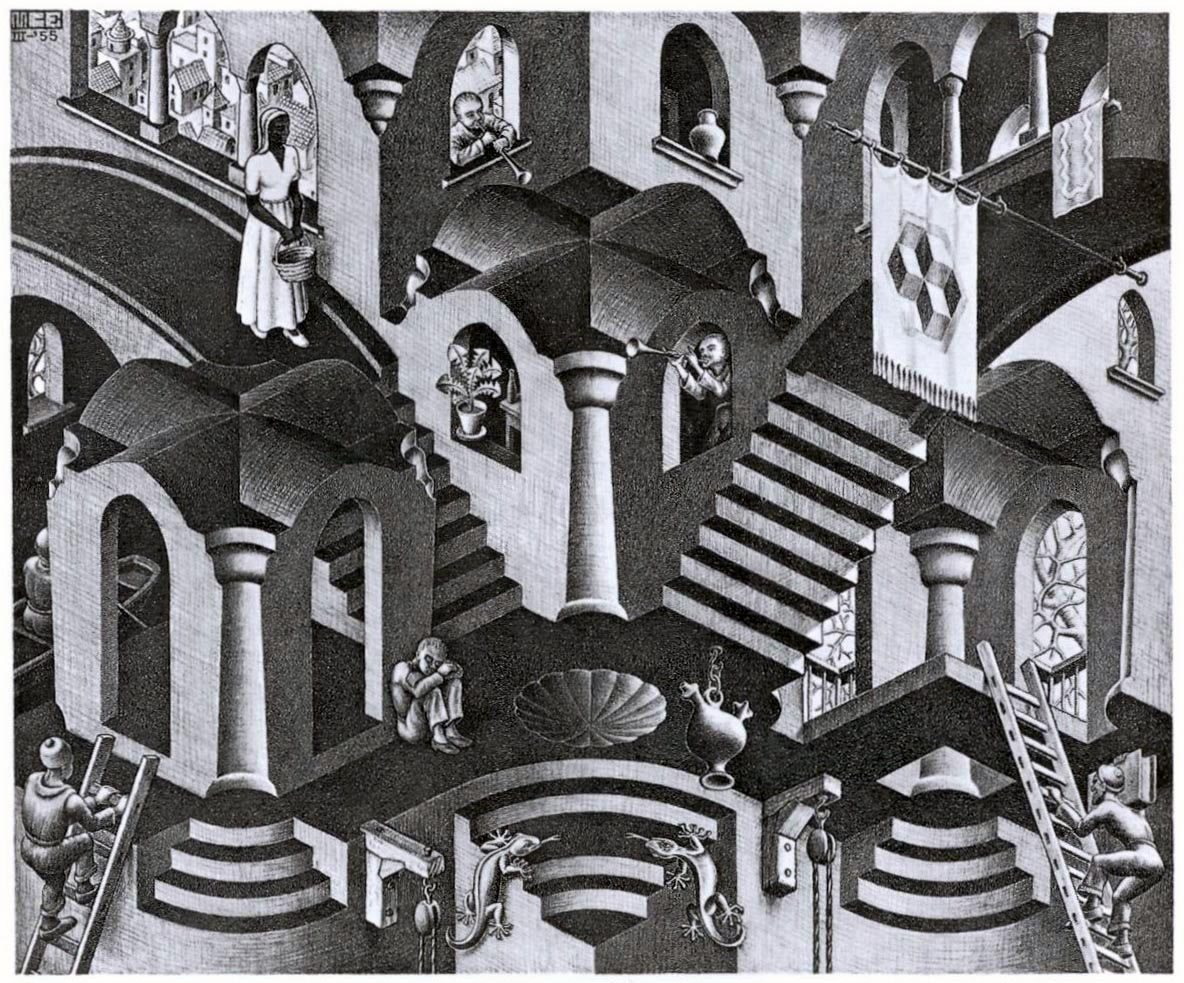
\includegraphics{img_023.jpg}
\caption[凹与凸,艾舍尔作。]
  {凹与凸,艾舍尔作(石板画,1955)。}
\end{figure}

    \item[乌龟]这很危险,我的朋友。我不愿意冒这个险。

    \item[阿基里斯]我只想试一次。

    \dnote{(他偷偷地靠近那盏灯,满以为不会弄醒睡在附近的那个小伙子。可是突然,他在一块奇特的贝壳形凹状地板上滑倒,跌出来掉进空中,东歪西倒的,他想随便够着什么,还想用一只手抓住那盏灯。由于他这么猛烈地摇晃,那两只蜥蜴“咝咝”叫着迅猛地朝他伸出了舌头,而他却吊在空中无法脱身。)}

    \item[阿基里斯]救——命——啊!

    \dnote{(一个女人正走下楼梯,呼喊声引起了她的注意,还惊醒了睡着的小伙子。后者弄清了是怎么回事之后,脸上露出了和善的微笑,向阿基里斯打手势,告诉他一切都会好的。他用一种奇怪的带有喉音的语言向高处窗户上的一对号手喊了句什么,然后,马上有奇异的声音奏响了,而且还彼此相呼应。那个睡意惺忪的小伙子指着蜥蜴,阿基里斯看到这音乐对它们有一种强烈的催眠作用。不一会儿,它们完全丧失了知觉。随后那个救命的小伙子对两个正沿着梯子向上爬的人喊话。他们俩把各自的梯子拿上来,伸到在空中被困的阿基里斯那里,构成一座桥,然后打手势让阿基里斯赶快爬下来。而阿基里斯却先小心地把挂着灯的链子从屋顶上的挂钩中脱出来,取下那盏灯,然后才从梯桥上爬下来,那三个小伙子让他脱了险。阿基里斯搂住他们,十分感激地同他们紧紧拥抱。)}

    \item[阿基里斯]嘿,龟兄,我怎么报答他们呢?

    \item[乌龟]我正好知道这三位勇敢的孩子喜欢喝咖啡,而就在这座城里有个地方,咖啡煮得没比了。请他们去喝杯咖啡吧!

    \item[阿基里斯]好极了!

    \dnote{(这样,通过一系列可笑的手势、微笑和个别字词,阿基里斯对这些小伙子表达了他的邀请。随后,他们五个一起走出来,走下一段陡楼梯,来到城里。他们来到一家吸引人的咖啡馆,在外面坐下来,要了五杯咖啡。在他们品呷时,阿基里斯记起了他带着的那盏灯。)}

    \item[阿基里斯]我都忘了,龟兄——我弄到了这盏魔灯!但是——它有什么魔力?

    \item[乌龟]哦,很普通——一种怪物。

    \item[阿基里斯]什么?你是想说你擦它时,就会出来一个怪物听你使唤?

    \item[乌龟]没错。你以为呢?天上掉馅饼吗?

    \item[阿基里斯]嗯,这是挺神的!我可以随心所欲,嗯?我总是希望我碰见这种事……

    \dnote{(阿基里斯轻轻地擦着刻在那盏黄铜灯表面上的大字“灯”……突然,冒出了一大股烟,从烟的形状中,五个朋友都辨认出那是一个精怪,鬼一般地立在他们上面。)}

    \item[怪物]你们好,我的朋友们——非常感谢把我的灯从邪恶的双蜥蜴手中救出来。

    \dnote{(怪物一边说着,一边把那盏灯拿起来,塞进隐藏在他那飘摆于灯外的长袍皱褶中的口袋里。)}

    作为对你这一英雄行为的感谢,我愿意代表灯向你提供实现你任意三个愿望的机会。

    \item[阿基里斯]真是活见鬼!你不觉得是这样吗,龟兄?

    \item[乌龟]我的确也这么想。来吧,阿基,说第一个愿望。

    \item[阿基里斯]唔!可我应该提什么愿望呢?哦,我知道了!这是我在第一次读《天方夜谭》时想过的(那是本由许多愚蠢的——也是叠套的——故事组成的集子)——我愿我有一百个愿望,而不是三个!真聪明,是吧,龟兄?我敢说你从没有想到过这种把戏,我总是想为什么故事中的那些大脑迟钝的人从没有自己这么试试。

    \item[乌龟]也许现在你会找到答案的。

    \item[怪物]很抱歉,阿基里斯,我不能满足元愿望。

    \item[阿基里斯]我愿你告诉我什么是“元愿望”!

    \item[怪物]可这是元元愿望,阿基里斯——我也不能满足你。

    \item[阿基里斯]什什什么?我一点也听不懂。

    \item[乌龟]你干嘛不把你最后那个请求换种说法,阿基?

    \item[阿基里斯]你想说什么?我干嘛要换?

    \item[乌龟]嗯,你刚才说“我愿……”,你既然只是在问一件事,干嘛不用问句?

    \item[阿基里斯]好吧,虽然我不明白为什么。告诉我,怪物——什么是元愿望?

    \item[怪物]就是关于愿望的愿望。我不能满足元愿望,我只能满足简单的普通愿望,比如想要十箱啤酒啦、月里嫦娥啦、两吨黄金啦、环球旅行啦。你明白吗——类似这样的简单事物。而我无法满足元愿望。\emph{造物神}不允许我这么做。

    \item[阿基里斯]\emph{造物神}?谁是\emph{造物神}?他为什么不让你满足元愿望?这看起来比你刚才提到的那些事要容易得多嘛。

    \item[怪物]嗯,这事挺复杂的,你为什么不来讲讲你那三个愿望呢?或者至少说一个,我不能总呆在这个世界里……

    \item[阿基里斯]哦,真糟糕。我真的希望有一百个愿望……

    \item[怪物]唉,我不愿看到任何人这么失望。而且,元愿望也是我最喜欢的一种愿望。让我想想我是否可以做点什么。请等一分钟。

    \dnote{(怪物从他袍子上的一簇皱褶里拿出一样东西,那东西看上去就像他拿走的那盏黄铜灯一样,只是这盏是用白银做的。以前的那盏上刻有“灯”字,而在这盏灯上同样的地方却刻有小一些的字“元灯”。)}

    \item[阿基里斯]那是什么?

    \item[怪物]是我的元灯……

    \dnote{(他擦擦元灯,它便冒出一股烟来。在翻滚着的烟云中间,他们全都看到了他们上面立着一个魔鬼般的形体。)}

    \begin{dialogue}
      \item[元怪物]我是元怪物。你叫我吗,怪物阁下?你有什么愿望?
    \end{dialogue}

    \item[怪物]我对你,元怪物阁下,以及\emph{造物神},有个特殊的愿望。我想请求暂时解除一切对愿望类型的限制,允许一个无类型愿望存在一段时间。你能俯准我这个愿望吗?

    \begin{dialogue}
      \item[元怪物]我会把它通过层层机构发送出去的,这没有问题。请等半分钟。

      \dnote{(这位元怪物以怪物两倍的速度从她袍子上的一簇襞褶里拿出一样东西,那东西看去就像那盏白银元灯一样,只是这盏是用黄金做的。以前的那盏上刻有“元灯”字样,而在这盏灯上同样的地方却刻有更小一些的字“元元灯”。)}

      \item[阿基里斯]\dlnote{(他的声音比以前高了八度)}那是什么?

      \item[元怪物]这是我的元元灯……

      \dnote{(她擦擦元元灯,它便冒出一股烟来。在翻滚着的烟云中间,他们全都看到了他们上面立着一个魔鬼般的形体。)}

      \begin{dialogue}
        \item[元元怪物]我是元元怪物。你叫我吗,元怪物阁下?你有什么愿望?
      \end{dialogue}

      \item[元怪物]我对你,元元怪物阁下,以及\emph{造物神},有个特殊的愿望。我想请求暂时解除一切对愿望类型的限制,请求允许一个无类型愿望存在一段时间。你能俯准我这个愿望吗?

      \begin{dialogue}
        \item[元元怪物]我会把它通过层层机构发送出去的,这没有问题。请等十五秒钟。

        \dnote{(这位元元怪物以元怪物两倍的速度从他袍子上的一簇皱褶里拿出一样东西,那东西看去就像那盏黄金元元灯一样,只是这盏是用……)}

        \par\nointerlineskip\medskip
        \begin{tikzpicture}[inner sep=0pt, decoration={markings,
          mark=between positions 0 and 1 step 0.1 with
            {\fill (0,0) circle (\dimexpr 2pt * \numexpr 11 - \pgfkeysvalueof{/pgf/decoration/mark info/sequence number}\relax / 10\relax);}}]
        \node[anchor=east] (O) at (\linewidth,0) {\{\emph{造物神}\}};
        \path[postaction=decorate] (0,15mm)  to [bend right=15] (O.center);
        \path[postaction=decorate] (0,-15mm) to [bend left=15]  (O.center);
        \end{tikzpicture}
        \par\nointerlineskip\medskip

        \dnote{(……旋回到元元元灯中来,元元怪物把它卷回他自己的袍子里,这一动作只有元元元怪物的一半那么快。)}

        你的愿望被批准了,元怪物阁下。
      \end{dialogue}

      \item[元怪物]谢谢你,元元怪物阁下,以及\emph{造物神}。

      \dnote{(这位元元怪物像所有比他更高的那些神怪一样,旋回到元元灯中去,元怪物把它卷回她自己的袍子里,这一动作只有元元怪物的一半那么快。)}

      你的愿望被批准了,怪物阁下。
    \end{dialogue}

    \item[怪物]谢谢你,元怪物阁下,以及\emph{造物神。}

    \dnote{(这位元怪物像所有比她更高的那些神怪一样,旋回到元灯中去,怪物把它卷回他自己的袍子里,这一动作只有元怪物的一半那么快。)}

    你的愿望被批准了,阿基里斯。

    \dnote{(从他说“请等一分钟”,到这时正好过了一分钟。)}

    \item[阿基里斯]谢谢你,怪物阁下,以及\emph{造物神}。

    \item[怪物]我很高兴通知你,阿基里斯,你可以有一个无类型愿望——这就是说一个愿望、一个元愿望、或一个元元愿望,你愿意有多少“元”都可以——甚至可以有无数多个(如果你愿意)。

    \item[阿基里斯]啊,非常感谢,怪物阁下,不过,我的好奇心给逗起来了。在我说出我的愿望前,你能不能告诉我谁——或者说什么——是“\emph{造物神}”?

    \item[怪物]行啊。“\emph{造物神}”是代表“\emph{造物神}—\emph{物}色的—\emph{神}怪”这个短语中几个词的词首字组合。“神怪”这个词一般指怪物、元怪物、元元怪物等等。这是个无类型词。

    \item[阿基里斯]可是——可是——这个由几个词的词首字组合而成的“\emph{造物神}”怎么会是一个词呢?这不会有任何意思!

    \item[怪物]噢,你没见过递归的词首字组合吗?我以为人人都知道呢。你瞧,“\emph{造物神}”代表“\emph{造物神}—\emph{物}色的—\emph{神}怪”——而它又可以被展成“\emph{造物神}—\emph{物}色的—\emph{神}怪—\emph{物}色的—\emph{神}怪”——它还可以依次被展成“\emph{造物神}—\emph{物}色的—\emph{神}怪—\emph{物}色的—\emph{神}怪—\emph{物}色的—\emph{神}怪”——它还可以依次被进一步展开……你可以想展多开就展多开。因为在每种情况下最前面的三个字总是“\emph{造物神}”,而这最前面的三个字总可以被展开。

    \item[阿基里斯]可我将永远不会展完!

    \item[怪物]当然不会。你永远也不会把“\emph{造物神}”全部展开。

    \item[阿基里斯]哼……真叫人费解。你对元怪物说“我对你,元怪物阁下,以及\emph{造物神},有个特殊的愿望”,这是什么意思呢?

    \item[怪物]我是想不仅向元怪物发出请求,而且也向她之上的所有神怪发出请求。递归词首字组合很自然地完成了这一任务。你瞧,当元怪物接受了我的请求时,她就不得不把它向上传给她的\emph{造物神}。所以她向元元怪物送去一个同样的信息,后者也照样对元元元怪物这么做……沿着这条链一直向上,就把信息传给了\emph{造物神}。

    \item[阿基里斯]我明白了。你的意思是说\emph{造物神}端坐在神怪之梯的顶端?

    \item[怪物]不,不,不!“顶端”一无所有,因为根本就没有顶端。这就是为什么\emph{造物神}是个递归的词首字组合。\emph{造物神}不是某个终极神怪。\emph{造物神}是个位于任何已知神怪之上的众神怪之塔。

    \item[乌龟]在我看来,每一个神怪都对\emph{造物神}是什么有彼此不同的看法,这样一来,由于对任何神怪来说,\emph{造物神}都是位于他或她之上的一组神怪,所以没有两个神怪具有同样的\emph{造物神}。

    \item[怪物]绝对正确——因为我是一切神怪中最低的,我可怜那些高层的神怪们,它们幻想着自己多少离\emph{造物神}更近些,多亵渎啊!

    \item[阿基里斯]乖乖,发明\emph{造物神}可真需要点儿神思。

    \item[乌龟]你真的相信关于\emph{造物神}的这些玩意儿吗,阿基?

    \item[阿基里斯]那当然啦。难道你是无神论者吗,龟兄?要不你就是个不可知论者。

    \item[乌龟]我不认为我是不可知论者。我也许是个元不可知论者。

    \item[阿基里斯]什什什么?我一点也听不懂。

    \item[乌龟]是这样……如果我是个元不可知论者,我就会为我是否是一个不可知论者而困惑——但是我并不清楚我是否是个元不可知论者;因此我一定是个元元不可知论者(我这么猜想)。啊,好啦。告诉我,怪物,神怪们犯过什么错误吗?在这条链上来回传递消息的时候,有过什么歪曲吗?

    \item[怪物]这种事确实有过。这是无类型愿望不被批准的最根本的原因。注意,这种歪曲在这条链上的任何一个个别环节发生的可能性都是无穷小的——但是当你把这无穷多种可能列出来,就能够清楚这样的歪曲一定会在某些地方发生。事实上,奇怪的是,经常会有无穷个歪曲,虽然它们在这条链上分布得很分散。

    \item[阿基里斯]这么说,能有什么无类型愿望被通过,那简直就是个奇迹了?

    \item[怪物]不。大多数歪曲不会造成严重后果,许多歪曲都互相抵消了。不过偶尔——事实上很少见——某种无类型愿望不能满足的原因可以追溯到某一个不幸的神怪所做的歪曲。一旦发生这种事,那个有罪的神怪就得被迫接受责罚,\emph{造物神}会鞭打他或她的屁股。对于执鞭者来说,这很有趣;对受笞者来说,也没多大害处。看到这一场面你会觉得挺逗的。

    \item[阿基里斯]我真想看看!不过只有在一个无类型愿望不被批准时才会有这种事,对吗?

    \item[怪物]正是。

    \item[阿基里斯]嗯……这给了我一个启发,是关于我的愿望的。

    \item[乌龟]噢,真的吗?什么启发?

    \item[阿基里斯]我希望我的愿望不被批准!

    \dnote{(就在这时,发生了一个无法描述的事件——用“事件”这个词行吗?——因此我们将不去描述它了。)}
  \end{dialogue}

  \item[阿基里斯]这个难以捉摸的解释究竟是什么意思?

  \item[乌龟]它是指阿基里斯说出的无类型愿望。

  \item[阿基里斯]可他还没说出来呢。

  \item[乌龟]他说了。他说:“我希望我的愿望不被批准”,而怪物把这当做是他的愿望了。

  \dnote{(就在这时,他们听到他们那一边的厅廊里有脚步声走来。)}

  \item[阿基里斯]哦,天呐!听起来可真不祥。

  \dnote{(脚步声停了,随后又转变了方向,并逐渐消失了。)}

  \item[乌龟\dlnote{(如释重负地)}]唉!

  \item[阿基里斯]故事说到哪儿了?这就是结尾吗?我们翻过这页看看。

  \dnote{(乌龟把《神怪和煮调饮》这页翻过去,他们发现故事在继续进行着……)}

  \begin{dialogue}
    \item[阿基里基]嗨!怎么回事?我的怪物哪儿去了?我的灯呢?我那杯咖啡呢?我那些从凹与凸的世界里来的朋友们怎么样了?那些小蜥蜴在这儿干什么呀?

    \item[乌龟]恐怕我们的环境恢复错了。

    \item[阿基里基]你这个难以捉摸的解释究竟是什么意思?

    \item[乌龟]我是指你说出的无类型愿望。

    \item[阿基里基]可我还没说出来呢。

    \item[乌龟]你说了。你说:“我希望我的愿望不被批准”,而怪物把这当做是你的愿望了。

    \item[阿基里基]哦,天哪!听起来可真不祥。

    \item[乌龟]这其实是个悖论。因为批准这个无类型愿望,就是否定了它——而不批准它,就是批准了它。

    \item[阿基里基]这会怎么样呢?地球会停止转动吗?宇宙会塌下来吗?

    \item[乌龟]不会,但是系统塌了。

    \item[阿基里基]什么意思?

    \item[乌龟]就是说你我,阿基,会忽然地、同时地被驱逐到堕界去。

    \item[阿基里基]到哪儿去?

    \item[乌龟]堕界:没有打出来的嗝和已熄灭的灯光所在的地方。它是一种候室,在这儿处于休眠的软件等着宿主硬件回来。无法知道这个系统要瘫痪多久,我们会一直呆在堕界里,也许几分钟,也许要几小时、几天——甚至几年。

    \item[阿基里基]我不知道软件是什么,我也不知道硬件是什么。不过我可知道我没有说出我的愿望!我想要怪物回来!

    \item[乌龟]很抱歉,阿基——是你闯的祸。是你搞垮了那个系统。我们能回来真得谢天谢地,不然后事情会变得更糟。不过我一点也不知道我们现在在哪儿。

    \item[阿基里基]我现在认出来了——我们在艾舍尔的另一幅画里。这回是《爬虫》。

\begin{figure}
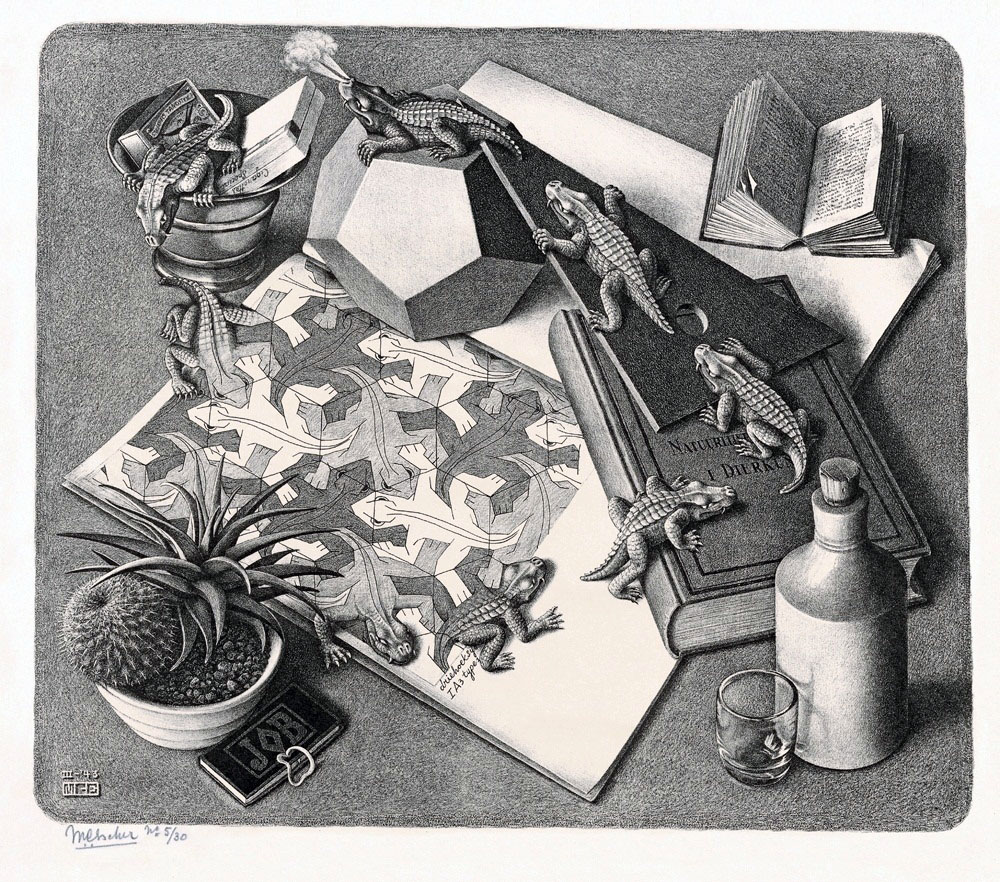
\includegraphics{img_024.jpg}
\caption[爬虫,艾舍尔作。]
  {爬虫,艾舍尔作(石板画,1943)。}
\end{figure}

    \item[乌龟]啊哈!系统在坍塌之前尽可能地努力保存我们的环境,它仅仅来得及记下我们是在艾舍尔的一幅有蜥蜴的画里,就完蛋了。也真为难它了。

    \item[阿基里基]瞧——那边桌子上不是我们的那瓶弹出煮调饮吗?就是在蜥蜴圈旁边!

    \item[乌龟]没错儿,阿基。我得说我们的确很幸运。系统把弹出煮调饮还给了我们,这对我们真是太好了——它对我们来说真是太珍贵了!

    \item[阿基里基]我也这么说!现在我们可以从艾舍尔的世界里弹回我的房子里了。

    \item[乌龟]煮调饮旁边还有两本书。什么书啊?\dlnote{(拿起小的那本,随便翻开一页。)}这书看起来挺吸引人的。

    \item[阿基里基]哦,真的?书名是什么?

    \item[乌龟]《乌龟和阿基里斯在全球各地转悠时的历险》。看样子读起来一定很有趣。我得好好看看——怪物和阿基里斯旅行的故事在哪儿?原来这本书有好几个层次,我得仔细找找。

    \item[阿基里基]好吧,你要想看就看吧,但是我可不想让那瓶弹出煮调饮冒险——没准儿哪只蜥蜴会把它碰下桌子,我现在就想把它拿到手!

    \dnote{(他冲到桌子前,伸手去拿那瓶弹出煮调饮,可是忙乱中,他大概是撞了那瓶子一下,瓶子翻倒了,掉下桌子开始滚起来。)}

    哦,哦!龟兄——你看!我不小心把那瓶子碰到了地板上,它朝——朝——楼梯滚去了!快——别让它掉下去!

    \dnote{(可乌龟这时完全沉浸在他手中的那本小薄书里去了。)}

    \item[乌龟]\dlnote{(喃喃地)}嗯嗯,看来在这一层里是找不到那种意思了。

    \item[阿基里斯]龟兄,龟兄,帮帮忙!帮忙抓住那个药瓶子!

    \item[乌龟]干嘛这么大惊小怪的?

    \item[阿基里斯]那只装煮调饮的瓶子——我把它从桌子上碰掉了,现在它正滚呢,它——

    \dnote{(这时它滾到了楼梯井的边缘,然后掉下去了。)}

    啊,可别!这可怎么办?龟兄——你怎么还跟没事一样?我们的药水没了!掉到楼梯下面去了!只有一个办法了,我们得下一层。

    \item[乌龟]下一层?没问题,请跟我来!

    \dnote{(他开始大声朗读,一时间阿基里斯进退两难,最后终于安定下来,充当了乌龟的角色。)}

    \begin{dialogue}
      \item[阿基里斯]这儿真黑,龟兄。我什么都看不见。吁!我撞在墙上了。当心!

      \item[乌龟]来——我这里有两只俄国手杖。拿上一根吧。你可以用它探路,这样你就不会碰东撞西了。

      \item[阿基里斯]好主意。\dlnote{(他拿了手杖。)}你觉出我们走的这条路有点往左拐吗?

      \item[乌龟]对,有一点点。

      \item[阿基里斯]我不知道咱们到哪儿了。我们还能重见天光吗?我当时真不该听你的,喝下了贴着“喝我”的那瓶东西。

      \item[乌龟]我向你保证这没什么不好。我干过无数次了,一次也没有后悔过。放松点,享受一下变小后的感觉。

      \item[阿基里斯]变小?龟兄,你都对我干了些什么呀?

      \item[乌龟]别怪我,你这样做是你自愿的啊。

      \item[阿基里斯]你把我缩小了吗?那么我们呆在其中的这个迷宫实际上是个小得可以被一脚踏过的玩意啦?

      \item[乌龟]迷宫?迷宫?可能吗?难道我们是在那个著名的由可怕的大雕所占据的和声小迷宫里吗?

\begin{figure}
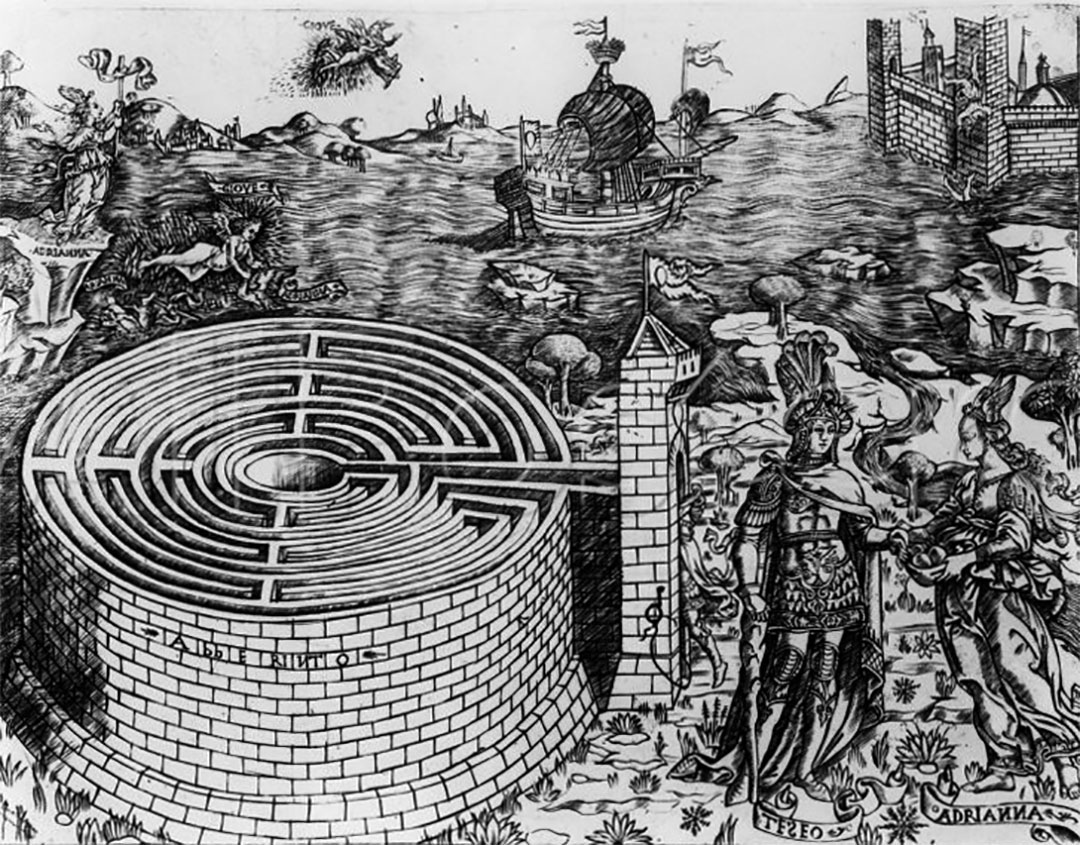
\includegraphics{img_025.jpg}
\caption[克里特迷宫。]
  {克里特迷宫(意大利蚀刻画:费尼盖拉派)[选自马修斯[W. H. Mathews]所著《迷津和迷宫——其历史及发展》[\bn{Mazes and Labyrinths: Their History and Development}]纽约:Dover Publications,1970年版。]}
\end{figure}

      \item[阿基里斯]天哪!那是什么?

      \item[乌龟]据说——我本人从不相信——一只邪恶的大雕造了一个小迷宫,自己居于它中间的一个小窝里,等待无辜的牺牲品在它那可怕的繁复通道之间转向。然后,当他们茫然失措地转悠到迷宫中心时,它就大笑不止,冲他们大笑——使劲地笑,直到把他们笑死!

      \item[阿基里斯]太可怕了!

      \item[乌龟]不过这只是个神话。勇敢些,阿基。

      \dnote{(这坚强的一对艰难地走着。)}

      \item[阿基里斯]摸摸这些墙。他们好像是有褶皱的锡板什么的。不过褶皱的大小不同。

      \dnote{(为了强调他的看法,他一边走,一边把那只俄国手杖伸出来抵着墙壁。当手杖在褶皱上来回弹跳时,在他们所在那条弯曲的长长走廊里,回响了奇特的声音。)}

      \item[乌龟\dlnote{(吃惊地)}]这是什么声音?

      \item[阿基里斯]噢,是我在墙上蹭我的手杖呢。

      \item[乌龟]哦!我以为是凶猛的大雕在叫唤呢!

      \item[阿基里斯]当然啦,没有什么可怕的。

      \dnote{(阿基里斯又把他的手杖蹭着墙,继续走着。这时可以听到他的手杖刮墙的地方发出了音乐声。)}

      \item[乌龟]嗯,我觉得不妙,阿基。那个迷宫也许根本就不是个神话。

      \item[阿基里斯]等等,是什么让你突然改主意了?

      \item[乌龟]你听到音乐了吗?

      \dnote{(为了听得更清楚些,阿基里斯放下了抬起的手杖,而那美妙的旋律也随之停止了。)}

      嗨!把手杖放回去!我想听听这段曲子的结尾!

      \dnote{(阿基里斯稀里糊涂地听从了乌龟的指令,音乐又继续下去了。)}

      谢谢,我刚才要说话的时候,突然明白我们在哪儿。

      \item[阿基里斯]真的?我们在哪儿?

      \item[乌龟]我们正沿着一张放在套子里的唱片上的纹沟走呢。你的手杖刮着墙上的那些奇形怪状的东西,就像是唱针沿着唱片的音纹转,就这样我们听到了音乐。

      \item[阿基里斯]哎呀,这可怎么办?这……

      \item[乌龟]怎么啦?你怎么不高兴?你以前有过这么密切地同音乐接触的机会吗?

      \item[阿基里斯]龟兄,我比个跳蚤还小,怎么还能有劲跑过身高正常的人呢?

      \item[乌龟]噢,就这点让你不安吗?根本不必为此发愁,阿基。

      \item[阿基里斯]看你说话的样子,我觉得你一点也不担心。

      \item[乌龟]我不知道,不过有一点可以肯定,我不担心没劲儿。尤其是在面临遇见大雕这种危险的时候。

      \item[阿基里斯]太可怕了!你是说——

      \item[乌龟]恐怕是的,阿基。我一听那段音乐就知道了……

      \item[阿基里斯]怎么回事?

      \item[乌龟]很简单。当我听到最高声部的B-A-C-H旋律时,我立刻听出我们正在穿行而过的这些音纹只能是《和声小迷宫》{}——巴赫的一首不太为人所知的管风琴作品。取这个名字是因为它那令人心醉神迷的频繁转调。

      \item[阿基里斯]什——什么玩意儿?

      \item[乌龟]嗯,你知道,大多数乐曲都用一个调或调性写成的。比如C大调,这只曲子就是C大调。

      \item[阿基里斯]我以前听说过这个词。它的意思是不是说你希望它结束在音符C上?

      \item[乌龟]对。在某种意义上说,C起一个“基底”的作用。实际上,通常叫它“主调音”。

      \item[阿基里斯]是不是离开了主调音就是为了最后回到主调音?

      \item[乌龟]正是这样。随着乐曲的发展,运用了模棱两可的和弦旋律,它们都离开了主调音。渐渐地,期待形成了——你越来越渴望回复,听到主调音。

      \item[阿基里斯]这就是为什么我在一支曲子结束时总是感到那么满足,就像我全身心都在等待着听到那个主调音似的,是吗?

      \item[乌龟]没错儿。作曲家运用他的和声进行来控制你的感情,使你产生渴望听到主调音的愿望。

      \item[阿基里斯]可是你该给我讲讲转调。

      \item[乌龟]哦,对。作曲家可以做的一件非常重要的事就是在一支曲子中“转调”,其目的在于建立一个暂时的终结,而不是一种主调音的解决。

      \item[阿基里斯]我想……我明白了。你是说某组用不同音调反复演奏的和弦改换了和声的紧张点,这样一来就使我实际上期待着在一个新的调上把不谐和音转变为谐和音?

      \item[乌龟]对极了。这就使情况更复杂了,因为虽然一时你期望在一个新调上把不谐和音转变为谐和音,但在你内心深处一直存在着一个渴望,即要达到原来那个终结——在这支曲子里就是大调的C。而当次要终结到达时,就会有——

      \item[阿基里斯\dlnote{(突然热情地打着手势)}]哦,听听这华美的突然上升的和弦,这是《和声小迷宫》结尾的标志。

      \item[乌龟]不,阿基,这不是结尾,这只是——

      \item[阿基里斯]它肯定是!喔!多么强有力的结尾啊!真让人有如释重负之感!这才是个解决呢!妙极了!

      \dnote{(确实,音乐就在这里停止了,他们走出来,到了一块没有墙壁的空地上。)}

      你瞧,它确实完了。我说什么来着!

      \item[乌龟]真邪了!这张唱片是音乐界的耻辱。

      \item[阿基里斯]什么意思?

      \item[乌龟]就是我刚告诉你的意思。这里巴赫从C调转到G调,建立起听G的第二个目的。这意味着你同时体验到两种张力——等待着向G转变,可同时心里还埋藏着那个最大的渴望——成功地转到C大调。

      \item[阿基里斯]你为什么听一支乐曲时一定要苦思冥想呢?音乐只是一种智力游戏吗?

      \item[乌龟]不,当然不是。某些音乐是极富于智慧的,不过大多数音乐不是。多数的时候你的耳朵或大脑为你“估算”,使你的情感知道它们想听什么,你不必有意识地去想它。但是在这支曲子里,巴赫在耍手腕,想把你引入歧途。而在你身上,阿基,他成功了。

      \item[阿基里斯]你是指我对副调解决的反应?

      \item[乌龟]正是。

      \item[阿基里斯]可我还是觉得它像个结尾。

      \item[乌龟]巴赫有意那么安排的。你恰好落入他的圈套了。它故意被设计得像个结尾,但是如果你仔细品味那个和声的进行,你会发现它的调性不对。显然,不只是你,连这个蹩脚的唱片公司也落入了同样的圈套——他们过早截断了这支曲子!

      \item[阿基里斯]巴赫可把我给涮了!

      \item[乌龟]这就是他的全部花招——让你在迷宫里迷路!大雕跟巴赫是同谋,你瞧,如果你不小心,他现在就会把你给笑死的——没准儿连我也给捎上呢。

      \item[阿基里斯]哦,让我们赶快离开这儿吧!快,咱们沿着音纹往回跑,在大雕发现我们之前跑出这张唱片!

      \item[乌龟]天哪,不行!我的感觉太脆弱,受不了倒序演奏时那古怪的和声进行。

      \item[阿基里斯]哦,龟兄,要是我们不能顺原路回去,我们怎么才能离开这里呢?

      \item[乌龟]是啊。

      \dnote{(阿基里斯有点绝望,开始在黑暗里乱跑。突然出现了一声轻微的喘息,接着“砰”地一声。)}

      阿基——你怎么了?

      \item[阿基里斯]有点错位,不过还好。我掉进了一个大洞里。

      \item[乌龟]你掉到邪恶大雕的窝里去啦!我在这儿呢,我来帮你出来。我们得赶紧走!

      \item[阿基里斯]小心,龟兄——我不想让你也掉进来……

      \item[乌龟]别怕,阿基,一切都会——

      \dnote{(突然间出现了一声轻微的喘息,接着“砰”地一声。)}

      \item[阿基里斯]龟兄——你也掉进来了!你怎么样?

      \item[乌龟]只是伤着了我的自尊心,不过还好。

      \item[阿基里斯]我们崴泥了,是吧?

      \dnote{(突然,一阵隆隆的笑声响起,并吓人地靠近了。)}

      \item[乌龟]当心,阿基,这可不是玩笑的事!

      \item[大雕]嘿嘿嘿!呵呵呵!哈哈哈!

      \item[阿基里斯]我开始顶不住了,龟兄……

      \item[乌龟]千万别理它的笑,阿基。这是你唯一的希望。

      \item[阿基里斯]我尽力而为吧。只要我的肚子不那么饿!

      \item[乌龟]哎,我闻到什么啦?附近有一碗弹出锅酥吧?

      \item[阿基里斯]我也闻到了。从哪儿飘来的?

      \item[乌龟]我想就在附近。哦!我碰在一个大碗一样的东西上了。对,没错儿——像是一大碗弹出锅酥。

      \item[阿基里斯]哦,天哪——弹出锅酥!我可得甩开腮帮子足吃!
    \end{dialogue}
  \end{dialogue}
\end{dialogue}

\item[乌龟]可别是推入锅酥!推入锅酥和弹出锅酥可真不好分清呀。

\begin{dialogue}
  \item[]
  \begin{dialogue}
  \item[]
    \begin{dialogue}
      \item[阿基里斯]焚琴?你说什么呢?

      \item[乌龟]我什么也没说呀。你大概是有点风声鹤唳了吧。

      \item[阿基里斯]还煮鹤!我真的不喜欢鹤肉。好啦,我们就吃这个吧!

      \dnote{(两个朋友开始大嚼弹出锅酥(或者推入锅酥?)——可突然——“弹”地一声!我猜他们吃的到底还是弹出锅酥。)}
    \end{dialogue}

    \item[乌龟]多有趣的故事啊。你喜欢它吗?

    \item[阿基里斯]一般。我想知道的只是他们离开那邪恶大雕的窝没有。可怜的阿基里斯——他想恢复正常身高。

    \item[乌龟]别担心——他们出去了,他也恢复了正常身高。这就是刚才为什么有一声“弹”。

    \item[阿基里斯]哦,我没听出来。嗯,我现在的确想找那瓶煮调饮了。不知为什么,我的嘴唇都要裂了。没有什么比弹出煮调饮更好喝的了。

    \item[乌龟]这种饮料以消燥解渴著名。在有些地方,人们对它着了魔。在十九世纪末、二十世纪初的维也纳,勋伯格食品工厂停止生产煮调饮,转产十二瓶菌氯,你无法想象由此而引起的骚乱。

    \item[阿基里斯]我略有所闻。不过还是让我们找找那瓶煮调饮吧,嘿——等一会儿。桌上这些蜥蜴——你发现它们有什么特别的吗?

    \item[乌龟]嗯——没什么特别的。你看见了什么这么有趣?

    \item[阿基里斯]你没看见?它们没喝什么弹出煮调饮就从那张平面上的画里跑出来了。它们怎么做到的?

    \item[乌龟]我没告诉你吗?要是你没有弹出煮调饮的话,你以同画面成直角的方向移动,也能从里面出来。这些小蜥蜴知道,要想从两维的画中世界里出来,就得向上爬。

    \item[阿基里斯]我们要从艾舍尔的这幅画中出来,也得做同样的事吗?

    \item[乌龟]当然!我们只需要上一层。你想试试吗?

    \item[阿基里斯]只要能回到我的房子里!这次吸引人的历险已经使我很累了。

    \item[乌龟]跟着我,从这条路上来。

    \dnote{(他们走上一层。)}
  \end{dialogue}

  \item[阿基里斯]可回来了。真好。不过有点不对劲儿。这不是我的房子!这是你的,龟兄。

  \item[乌龟]唔,是的——我倒愿意这样呢!我一点也不想从你那里再走那么长的路回来了。我累坏了,简直怀疑我是否走了那么远。

  \item[阿基里斯]我不在乎走回家,所以我想我们在这儿结束也挺好。

  \item[乌龟]说得对!这的确是次好运!

\end{dialogue}
\end{dialogue}

\end{dialog}
